\documentclass{beamer}
\usepackage{listings}
\lstset{
%language=C,
frame=single, 
breaklines=true,
columns=fullflexible
}
\usepackage{blkarray}
\usepackage{subcaption}
\usepackage{url}
\usepackage{xurl}
\usepackage{tikz}
\usepackage{tkz-euclide} % loads  TikZ and tkz-base
%\usetkzobj{all}
\usetikzlibrary{calc,math}
\usepackage{float}
\newcommand\norm[1]{\left\lVert#1\right\rVert}
\renewcommand{\vec}[1]{\mathbf{#1}}
\usepackage[export]{adjustbox}
\usepackage[utf8]{inputenc}
\usepackage{amsmath}
\usepackage{amssymb}
\usepackage{wrapfig}
\usepackage{bm}
\usepackage{tikz}
\setbeamertemplate{caption}[numbered]
\usetikzlibrary{automata, positioning}
\usetheme{Boadilla}
\providecommand{\pr}[1]{\ensuremath{\Pr\left(#1\right)}}
\providecommand{\sbrak}[1]{\ensuremath{{}\left[#1\right]}}
\providecommand{\lsbrak}[1]{\ensuremath{{}\left[#1\right.}}
\providecommand{\rsbrak}[1]{\ensuremath{{}\left.#1\right]}}
\providecommand{\pr}[1]{\ensuremath{\Pr\left(#1\right)}}
\providecommand{\brak}[1]{\ensuremath{\left(#1\right)}}
\providecommand{\lbrak}[1]{\ensuremath{\left(#1\right.}}
\providecommand{\rbrak}[1]{\ensuremath{\left.#1\right)}}
\providecommand{\cbrak}[1]{\ensuremath{\left\{#1\right\}}}
\providecommand{\lcbrak}[1]{\ensuremath{\left\{#1\right.}}
\providecommand{\rcbrak}[1]{\ensuremath{\left.#1\right\}}}

\title{Research Paper Presentation}
\author{Shashank Shanbhag}
\date{CS20BTECH11061}
\begin{document}

\begin{frame}
\titlepage
\end{frame}

\begin{frame}
    \begin{block}{Title}
    Machine to Machine Based on Visible Light Communication for IoTs.
    \end{block}
    \begin{block}{Authors}
    \begin{itemize}
        \item Rodrique Chi Fon
        \item Alain R. Ndjiongue
        \item Khmaies Ouahada
        \text{All of them are Professors in Dept. of Electrical and Electronic}
        \text{Engineering Science, University of Johannesburg, South Africa.}
    \end{itemize}
    \end{block}
\end{frame}

\begin{frame}
  \frametitle{}
  \begin{block}{Pre-requisites}
    \begin{itemize}
        \item Heterogeneous network 
        \item Visible light communication (VLC)  
        \item Machine-to-machine (M2M) VLC
        \item Modulation
        \item Internet of Things (IoTs)
        \item Signal Noise Ratio (SNR)
        \item On-Off Keying (OOK) 
        \item Additive white Gaussian noise (AWGN)
        \item Bit Error Rate (BER)
        \item Line Of Sight(LoS)
        \item Handover
    \end{itemize}
  \end{block}
\end{frame}

\begin{frame}
  \frametitle{}
  \begin{block}{Heterogeneous network}
    \textbf{Heterogeneous network} means wireless network.
  \end{block}
   \begin{block}{Visible light communication (VLC)}
   \textbf{VLC} is a data communication variant which uses visible light for data transmission, providing both lighting and high speed wireless access. It is a subset of optical wireless communication (\textbf{OWC}) technologies.
  \end{block}
  \begin{block}{Machine-to-machine (M2M) VLC}
    \textbf{M2M VLC} is a communication architecture that makes it possible for heterogeneous devices to interact without human intervention using visible light modulated at certain frequency to enable communication.
  \end{block}
  \begin{block}{Modulation}
  \textbf{Modulation} means the process of changing the amplitude or frequency of an electric signal by mixing it with another signal.
  \end{block}
\end{frame}

\begin{frame}
  \frametitle{}
  \begin{block}{IoTs}
  \textbf{IoTs} describes the network of physical objects (things) that are embedded with sensors, software, and other technologies for the purpose of connecting and exchanging data with other devices over internet.
  \end{block}
  \begin{block}{Signal Noise Ratio (SNR)}
  \textbf{SNR} ratio means the ratio of power of signal to power of background noise.
  \end{block}
  \begin{block}{OOK}
  \textbf{OOK} denotes the simplest form of converting digital data as variations in amplitude of a carrier wave to detect presence or absence of carrier wave. Ex: 1 for transmitting carrier wave and 0 for not transmitting.
  \end{block}
\end{frame}

\begin{frame}
  \frametitle{}
  \begin{block}{AWGN}
  \textbf{Additive white Gaussian noise (AWGN)} is a tool used to mimic random processes in nature.
  \end{block}
  \begin{block}{BER}
  \textbf{BER} is number of bit errors per unit time.
  \end{block}
  \begin{block}{LoS}
  \textbf{LoS} is a type of propagation that can transmit and receive data only where transmit and receive stations are in view of each other without any obstacle between them.
  \end{block}
  \begin{block}{Handover}
  \textbf{Handover} is a process in which cellular transmission (voice or data) is transferred from one base station (cell site) to another without losing connectivity to the cellular transmission.
  \end{block}
\end{frame}

\begin{frame}
  \frametitle{Some Images to illustrate definitions}
  \begin{columns}
	\begin{column}{0.48\textwidth}
		\begin{figure} [h]
    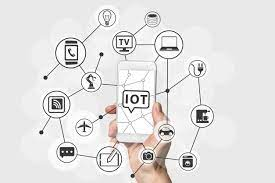
\includegraphics[width = 0.8\textwidth]{IoTs.jpg}
     \caption{IoTs}
        \end{figure}
	\end{column}
	\begin{column}{0.48\textwidth}
	\begin{figure} [h]
    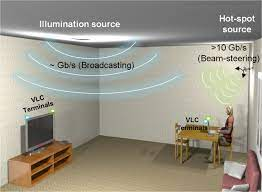
\includegraphics[width = 0.8\textwidth]{VLC.jpg}
    \caption{VLC}
    \end{figure}	
	\end{column}
\end{columns}
    \begin{figure} [h]
        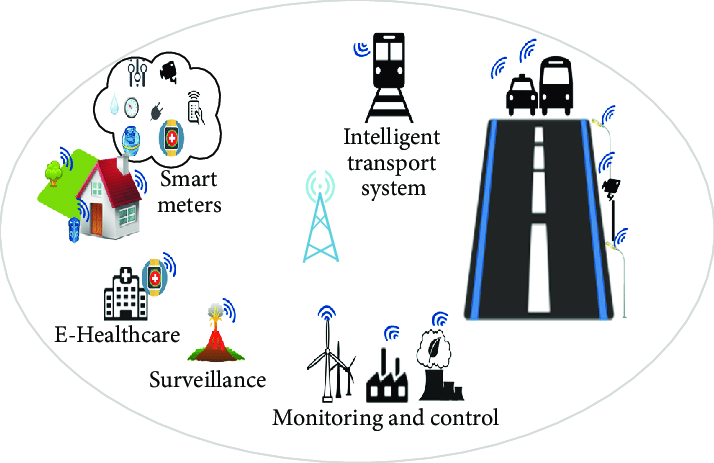
\includegraphics[width = 0.35\columnwidth]{M2M.PNG}
        \caption{M2M}
    \end{figure}
\end{frame}

\begin{frame}
  \frametitle{}
  \begin{block}{Why new technology?}
  The exponential increase in the number of devices that require internet services due to (M2M) and (IoTs). We now use \textbf{Radio frequency (RF)} wireless technologies like Wi-fi, Bluetooth with limitations of frequency spectrum, power usage and high rate of energy consumption. 
  \end{block}
  \begin{block}{Expectations}
  Better connectivity, High SNR, High data speed.
  \end{block}
  \begin{block}{Solution}
  The paper proposes VLC. Here we use LED’s to provide a light signal which is modulated at high speed to carry information, in addition to it lower power consumption. Also it has advantages like wide spectrum as well as readily available spectrum, less interference and harmless to humans. It can completely replace RF.
  \end{block}
\end{frame}

\begin{frame}
  \frametitle{}
  \begin{block}{Applications}
  \begin{itemize}
      \item Smart home
      \item Smart office
      \item Remote monitoring
      \item Vehicle-to-Vehicle communication(V2V)
      \item Digital signage
      \item Wireless sensor network
      \end{itemize}
      All the applications of IoTs are targeted mainly.
  \end{block}
\begin{columns}
	\begin{column}{0.48\textwidth}
		\begin{figure}[h]
    \includegraphics[width = 0.8\textwidth]{Smarthome.jpg}
    \caption{Smart Home}
        \end{figure}
	\end{column}
	\begin{column}{0.48\textwidth}
	\begin{figure} [h]
    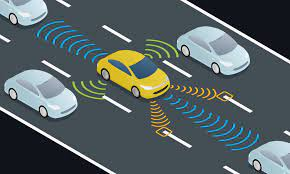
\includegraphics[width = 0.8\textwidth]{v2v.jpg}
    \caption{V2V}
    \end{figure}	
	\end{column}
\end{columns}
\end{frame}

\begin{frame}
  \frametitle{How does M2M VLC based system work?}
  \begin{block}{}
  \begin{itemize}
      \item As VLC is a part of OWC, so it has all the properties of OWC. VLC is consisted of three main parts, transmitter, channel and receiver and often characterized by additive white Gaussian noise (AWGN).
      \item To facilitate M2M communications with VLC, machine-type-communication devices must be connected to VLC access points.
      \item VLC’s short range transmission can be tackled by cascading with backbone networks such as laser, power line communication, fiber optics.
      \item The channel is the space from the transmitter antenna (LEDs) to the receiver antenna (PD)
      \item The channel could be characterized as single or multiple channels. Single channels are such that only one LED and one PD are utilized. Multiple channels are when there exist multi-colored LEDs
  \end{itemize}
  \end{block}
\end{frame}

\begin{frame}
  \frametitle{How does M2M VLC based system work?}
	\begin{figure} [h]
    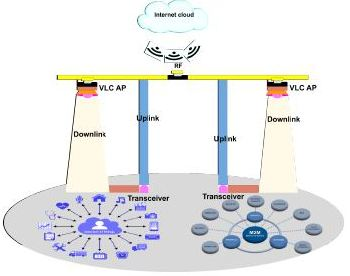
\includegraphics[width = 0.7\textwidth]{Fig1.jpg}
    \caption{A multi-channel VLC access system based on an indoor scenario.}
    \end{figure}	
\end{frame}

\begin{frame}
  \frametitle{How does M2M VLC based system work?}
	\begin{figure} [h]
    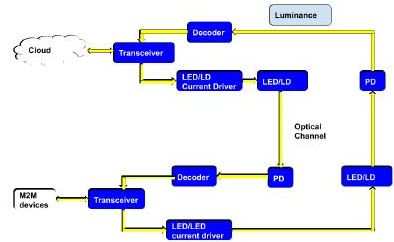
\includegraphics[width = 0.7\textwidth]{Fig2.jpg}
    \caption{A block diagram for M2M VLC based channel model for indoor and outdoor scenario}
    \end{figure}	
\end{frame}

\begin{frame}
  \frametitle{}
  \begin{block}{VLC for Outdoor environment}
  \begin{itemize}
      \item We propose our analysis based on an amplify forward (AF) strategy, where no processing of data is involved, in case of re-transmission.
      \item The light signals are detected and directly converted to a corresponding current and to the power of the LEDs or LDs.
      \item Considering that sunlight is principal source light, we model the system with a Gaussian normal distribution.
        \begin{equation}
         S_0 = H_0 S + N_0
        \end{equation}
        where S is the original message, $S_0$ is the message at the LD receiver and $N_0$, AWGN.
        \item For outdoor environment such as vehicle-to-vehicle communication, , only LoS is considered. This is because the power due to the NLoS is negligible when compared with the power from LoS part.
  \end{itemize}
  \end{block}
\end{frame}

\begin{frame}
  \frametitle{}
  \begin{block}{}
  \begin{itemize}
  \item The outdoor part is a single mode Gaussian beam stochastic-channel governed by
        \begin{equation}
            H_{LoS(o)} = \frac{2 A_l e^{-\gamma L}}{\pi \theta^2 L^2 }
        \end{equation}
   where $A_l$ is the effective laser receiver area, $\theta$ is the small angle beam divergence, L is the transmission range and $\gamma$ is the intensity of the attenuation coefficient.
  \end{itemize}
    \end{block}
\begin{block}{VLC for indoor channel}
\begin{itemize}
    \item In an indoor environment, such as office, smart homes, both line-of-sight (LoS) and non-line-of-sight (NLoS) are considered. 
    \item The indoor channel assumes the additive white Gaussian response while taking into consideration the non-line-of-sight (NLoS)
    \begin{equation}
         S_i = H_i S + N_i
        \end{equation}
    where S is the original message, $S_i$ is the message at the LED receiver and $N_i$ AWGN.
\end{itemize}
\end{block}
\end{frame}

\begin{frame}
  \frametitle{}
  \begin{block}{}
  \begin{itemize}
      \item The transfer function of the M2M VLC based indoor system is the summation of the LoS and NLoS links, which is a complicated mathematical expression.
  \end{itemize}
    \end{block}
    \begin{columns}
	\begin{column}{0.48\textwidth}
		\begin{figure}[h]
    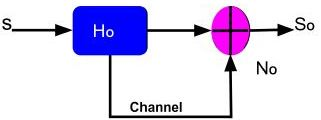
\includegraphics[width = 0.8\textwidth]{Fig3.jpg}
    \caption{Simplified channel modeled of LD systems in an outdoor environment}
        \end{figure}
	\end{column}
	\begin{column}{0.48\textwidth}
	\begin{figure} [h]
    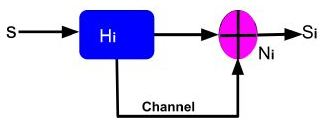
\includegraphics[width = 0.8\textwidth]{Fig4.jpg}
    \caption{Simplified channel modeled of LED systems in an indoor environment}
    \end{figure}	
	\end{column}
\end{columns}
\end{frame}

\begin{frame}
  \frametitle{Simulation results}
		\begin{figure}[h]
    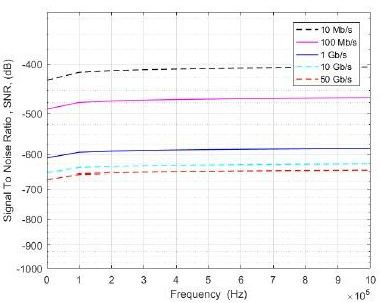
\includegraphics[width = 0.6\textwidth]{Fig6.jpg}
    \caption{Average received SNR for multiple values of the bit rate B of the channel against frequency.}
        \end{figure}
\end{frame}

\begin{frame}
  \frametitle{Simulation results}
  \begin{figure} [h]
    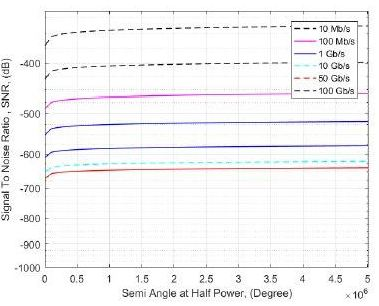
\includegraphics[width = 0.6\textwidth]{Fig7.jpg}
    \caption{Average received SNR for multiple values of the bit rate B of the channel against semi angle at half power.}
    \end{figure}
\end{frame}

\begin{frame}
  \frametitle{Simulation parameters}
  \begin{figure} [h]
    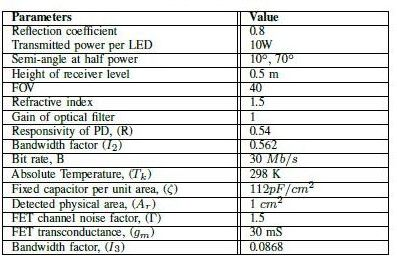
\includegraphics[width = 0.6\textwidth]{Fig5.jpg}
    \caption{Parameters used in simulation experiment}
    \end{figure}
\end{frame}

\begin{frame}
  \frametitle{Conclusion}
  \begin{itemize}
      \item The paper proposed a machine type communication (MTC) for M2M VLC based with an incorporation of energy harvesting system using a power transfer unit (PTU) with a centralized VLC access point (AP) with a probabilistic model, where an investigation is performed to show the signal to noise ratio (SNR) distribution with a semi angle at half power of a chosen link.
      \item M2M VLC based presents one of the most reliable secured and viable communication in IoTs with a proven tract of releasing high data rates and serves as a solution to already congested, overcrowded electromagnetic spectrum.
  \end{itemize}
\end{frame}

\end{document}

